%%=========================================
\section[Introduksjon]{Introduksjon}
%%=========================================
\subsection{Bakgrunn}

\subsubsection{Smarte hjem}
Definisjon. Behovet for smarte hjem: informasjon, læring, kommunikasjon, energieffektivitet, støtte av eldre.

Ideén om et smart hjem refererer i følge \citet{peine08} til å bruke informasjons- og kommunikasjonsteknologi (IKT) i hjemmet for å forenkle interoperabilitet av husholdningsprodukter og tjenester. Peine skriver at ideén har vært beskrevet siden 80-tallet og har i de senere år fått en ny interesse i industrien. Faktisk har kontroll av funksjonaliteten i en kontorbygning eksistert siden 70-tallet, med muligheter for å kontrollere lys, varme, elektristet og adgangskontroll fra et sentralt sted. Det tok noen år før man innså at de samme egenskapene kunne være ønskelige å implementere for å automatisere hus. Den sentrale forskjellen mellom et vanlig hus og smart hus er denne muligheten for å styre flere aspekter ved huset gjennom en sentral enhet.

På markedet finnes det nå flere løsninger for å automatisere deler av hjemmet eller tilby gode brukergrensesnitt for å styre funksjonalitet som lys og varme. Disse løsningene bidrar med å ivareta sikkerhet og hjelper til å begrense energiforbruket. De tilbyr gjerne informasjon om hjemmet via en mobilapplikasjon så man kan ha oversikten selv når man er bortreist. Ved å benytte enheter som er tilknyttet internettet, som termostater, lys, låser, sikkerhetssystemer og garasjeporter, kan man styre dem gjennom mobilapplikasjonen\footnote{Et søk i Google på "smarthome" og norske resultater gir for eksempel denne hjemmesiden der en privatperson har tatt i bruk og satt sammen komponenter fra markedet for å skape en helhetlig og gjennomført løsning: http://www.samdal.com/SmartHome.htm}. Disse løsningene er svært praktiske og gir god verdi, men er økt tilgang til informasjon og muligheten til å fjernstyre noen deler av hjemmet det beste vi kan få til i dag?

I en artikkel for Scientific American i 1991 skrev Mark Weiser at de mest dyptgripende teknologiene er de som forsvinner inn i hverdagslivet inntil det er umulig å skille dem ut igjen. Han så for seg at omgivelsene var gjennomtrengt med teknologi for databehandlig og kommunikasjon, og som kunne støtte opp under menneskers liv gjennom såkalt \emph{calm computing} \citet{weiser91}. Dette framtidssynet har styrt utviklingen for forskningsområdene \emph{pervasive/ubiquitous computing} og det peker mot de egenskapene og mulighetene et smart hjem bør tilby. Men hvorfor er ikke smarte hjem smarte nok til å tilby dette framtidssynet ennå? Det har godt mange år og det har blitt gjort mye arbeid siden 1991. Trolig har vi all del-funksjonaliteten som trengs for å implementere dette framtidssynet. Vi har kraftige innebygde enheter, sensorer på størrelse med frimerker, trådløs kommunikasjon, internettet og muligheten til å programmatisk kontrollere elektriske apparater, varme og lys. Vi kan analysere bilder og lydsignaler, gjenkjenne fjes og tale, overvåke og følge brukerenes bevegelser, samt koble oss opp mot eksterne datakilder som værmeldinger og brukerenes kalendere. Grunnen til at vi ikke har disse systemene ennå må være at det er vanskelig å sette det hele sammen og å gjøre god bruk av alle dataene som samles inn. Kunstig intelligens kan være nøkkelen for å gjøre teknologiene vi har om til nyttige tjenester.

For å forstå omgivelsenens tilstand vil det være nødvendig å analysere sensorinformasjon. To lovende input-kanaler er lyd og bilde. Ettersom vi mennesker kommuniserer med tale er det naturlig at et AmI-system skal kunne håndtere dette. Talegjenkjenning er et vanskelig problem, men det er et område det er jobbet mye med opp gjennom årene. Ved bruk av teknikker fra signalprosessering og mønstergjenkjenning kan man identifisere \emph{fonemer} i signalet og deretter ord. Tilsvarende kan man få en datamaskin til å utnytte seg av syn ved å få tak i input som bilder. Disse må også prosesseres og mennesker må gjenkjennes. I følge \citet{augustonugent06} kan datasyn kan være nyttig for å gjenkjenne mønstre i menneskers oppførsel eller oppdage når noe galt har skjedd, som at en eldre beboer har falt. Det kan også brukes til å gjenkjenne gesturer eller å gjenkjenne fjesuttrykk i et forsøk på å forstå brukerenes følelser. Dersom datasyn skal brukes vil det være viktig å skille beboeren fra besøkende, dyr eller andre bevegelige objekter. Å holde en historie over beboerens siste bevegelser kan hjelpe til med å forstå og avgjøre tilstander.

Et virkelig smart hjem kan lære av å observere brukere. Teknikker fra maskinlæring, som nevrale nettverk, case-based resonnering og beslutningstrær og støttevektormaskiner er godt utviklet og kan benyttes til dette. Å lære brukernes oppførsel vil være essensielt for at system skal forbedre seg selv over tid, og for å tilby en individuelt tilpasset opplevelse. Forskjellige brukere vil ha forskjellige tilstander, preferanser og vaner, og disse bør tas med i beregningen for at systemet skal være verdifullt.

Data som hentes fra hjemmet kan være interessant for forskjellige brukere, men hvilken informasjon skal hver person motta? Her kommer privathet og sikkerhet inn i bildet. Hvordan og til hvilket tidspunkt tar vi kontakt med brukeren? Uønsket eller unødvendig hjelp er sannsynligvis verre enn ingen hjelp. Påminnelser om oppgaver med lav prioritet kan være frustrerende. Vi ønsker kanskje heller ikke at brukere blir overavhengige av systemet, selv hvis det fungerer godt. For mange brukere kan dette peke mot at vi ønsker et minimalt nivå av hjelp. Dette vil la beboern ta i bruk sin egen kognitive kapasitet og vedlikeholde et høyt nivå av uavhengighet. 


\subsubsection*{Hva ønsker brukerne}
Ettersom vi snakker om hvorfor og hvordan man vil utvikle løsninger for å skape smarte hjem kan det være en god idé å ha kontakt med brukermassen. Smarte hjem er et relativt nytt produkt for det store markedet, så det er ikke sikkert at brukerene vet hva de vil ha fra et smart hjem, eller om de vil ha et smart hjem i det hele tatt. Men ettersom dette kan sees på som utviklingen av et nytt produkt vil det allikevel være klokt å ta pulsen på framtidige kunder. I stedet for å dytte behov på brukeren kan det være bedre å støtte opp under brukerens faktiske behov. Dette kan hjelpe oss å bygge produkter som blir godt motatt og dermed kan vi framskynde innføringen av smarte og automatiserte hjem.

\citet{bonino11} ledet en interessant italiensk studie som spurte en gruppe hva de ville spurt hjemmet sitt dersom det var intelligent. Studien viser at folk flest har sterke følelser knyttet til hjemmet. Det er et trygt og koselig sted. Det er et sted til å stole på og følelsen av å returnere dit er god. Generelt er å føle seg bra en del av hjemopplevelsen. Atmosfæren er behagelig og tilpasset brukerens preferanser og folk liker at de kan gjøre hva de selv vil. Brukere har følelsen av å være i kontroll.

Artikkelen presenterer hva gruppen mener er de viktigste områdene for det smarte hjemmet:
\begin{itemize}
  \item Intelligente brukergrensesnitt på hvitevarer, for eksempel stemmekontrollerte oppvaskmaskiner.
  \item En tilgjengelig klokke, for planlegging av aktiviteter.
  \item Tilgang til værinformasjon, da ønskede fritidsaktiviteter ofte avhenger av været utendørs.
  \item Ivaretagelse av egen sikkerhet og husets sikkerhet. Innbruddsbeskyttelse og automatisk oppdagelse av farer, som røyk-, varme- eller gassutvikling.
  \item Informasjon om energiforbruk og forslag til hvordan energiforbruket kan reduseres.
  \item Kontroll av husets underholdningssenter.
  \item Tilgjengelig kommunikasjonsbehov som å lese epost og bruke telefon.
  \item Automatisk oppdagelse og eventuell reparasjon av problemer.
  \item Husholdningsoppgaver som hjelp med oppgaver til å holde huset rent og komfortabelt, håndtering av mat og hjelp med planlegging av innkjøp.
  \item Komfortrelaterte problemer som lysregulering, temperaturregulering og operering av vinduer og persienner.
  \item Personlig assistanse, som å be huset om hjelp til å huske ting, søke opp informasjon og håndtere andre dagligdagse oppgaver.
\end{itemize}

En annen studie av brukerbehovene for smarte hjem presenteres av \citet{userreq}. Her omtales en empirisk studie utført på seks forskjellige steder i fem europeiske nasjoner. Studien bruker en scenario-drevet tilnærming og brukte kvantitative og kvalitative metoder for å få tilbakemelding fra brukermassen om konsepter innen smarte hjem. Deltakerene kom opp med en rekke forslag og ideer til hva et smart hjem bør tilby og prioriteringsrekkefølgen for disse funksjonalitetene. Generelt ble det funnet godt med beviser på hva brukere er interessert i: Systemet skal være lett å bruke og å konfigurere. Det skal ikke kreves programmering eller vedlikehold av noe slag. Systemet skal være modulært og tilby å justere for individuelle preferanser. Alle deltakerene var enig om at personvernet ikke måtte brytes gjennom overvåking. Den følgende listen er sortert med høyeste prioritet først.
\begin{enumerate}
  \item Brukeren må alltid være i kontroll av systemet.
  \item Systemet må ivareta sikkerhet, og beskytte personvernet.
  \item Et nytt system må gi ny verdi over eksisterende systemer.
  \item Systemet må ikke unødvendig overta rollen til direkte kommunikasjon mellom mennesker.
  \item Hjemmekomforten skal alltid ivaretas.
  \item Systemet skal tilby passende informasjon til passende brukere på forskjellige lokasjoner basert på brukerpreferanser.
  \item System skal redusere tiden som trengs for å utføre husholdningsoppgaver som vasking.
  \item Systemet skal integrere og kombinere funksjonaliteten til hvitevarer.
  \item Systemet skal være energibesparende.
  \item Systemet skal være kostnadsbesparende.
  \item Systemet skal støtte organiseringsaktiviteter og planlegging for flere personer i hjemmet, mellom forskjellige hjem og mellom hjemmet og jobb.
  \item Systemet skal beskytte mot datatyveri og annen manipulering (se punkt 2).
  \item Systemet skal tilby adgangskontroll og respektere individuelle preferanser og autoriteter.
  \item Systemet skal holde informasjon om kontekst og omgivelsene.
  \item Systemet skal forholde seg til implisitte sosiale normer.
  \item Systemet skal beskytte personvernet til enhver tid (se punkt 2).
\end{enumerate}

\subsubsection*{Støtte av eldre og funksjonshemmede}
Smarte hjem ønsker å tilby funksjonalitet relatert til gevinst innen økonomi og komfort, som at lys og varme skrues av og på automatisk avhengig av beboernes tilstedeværelse. Men det kan argumenteres for at den viktigste funksjonaliteten er for å forbedre en uavhengig livsstil for eldre og funksjonshemmede. Basert på antallet artikler om teamet må å opprette støtte for at eldre og funksjonshemmede skal få leve uavhengig i lengre tid være en av de mest studerte tilnærmingene til smarte hjem. En god grunn er at dette er den gruppen mennesker som vil ha størst nytte av et smart hjem. Muligheten til å fortsette å leve uavhengig og selvstendig i sitt eget hjem, framfor å bli innlagt på en institusjon, er virkelig verdifull. Et smart hjem kan hjelpe til med funksjonalitet som å gi påminnelser om at medisin må tas og å oppdage dersom noe har gått galt og automatisk ta kontakt med hjelpetjenester eller familie.

Den andre gode grunnen til at denne tilnærmingen studeres mye er på grunn restriksjonene denne beboergruppen har i sitt levesett. Når de forskjellige aktivitetene beboerne utfører kan telles på noen få hender blir det store problemet om å få et datasystem til å forstå menneskelige aktiviteter mye enklere. Det blir satt restriksjoner på problemet som gjør at det faktisk kan løses. Å løse problemet uten restriksjoner kan vise seg å være en svært vanskelig og kanskje umulig oppgave. Vi mennesker gjør ofte flere aktiviteter på en gang, samarbeider med andre mennesker og vi kan avslutte aktiviteter midtveis.


\citet{desilva12} påpeker at for systemene som fokuserer på støtte av eldre og funksjonshemmede er det ekstra viktig å detektere mennesker, ettersom en av hovedfunksjonalitetene til et slikt system er å gjenkjenne hvilken tilstand beboeren er i. Dersom beboeren for eksempel har falt er det viktig å gjenkjenne objektet på bakken som et menneske og ikke som en livløs gjenstand. Ettersom å gjenkjenne mennesker er av høyeste prioritet benytter mange av prosjektene i denne kategorien videoovervåkning. Når det gjelder deteksjon av fall skriver \citet{elliot09} om bruken av en pendel, refleksjons-sensorer og et nevralt nettverk for å følge pendelens posisjon i reell-tid. Resultatene indikerte at teknikken er tilstrekkelig sensitiv og kan brukes til å gjenkjenne forskjellene mellom en person som finner balansen og en som er i ferd med å falle. På denne måten kan hjemmet gjenkjenne og potensielt forhindre et fall før det skjer.

Casattenta-prosjektet gjør bruk av utplasserte sensorer, \emph{monitoring nodes}, fordelt i hjemomgivelsene, samt bærbare enheter, \emph{active keys}, for å overvåke beboernes helse og aktivitet (se figur \ref{casattenta}). \citet{casattenta} skriver at målet er å tilby tilstrekkelig, men ikke-påtrengende, overvåkning for å forbedre sikkerheten og livskvaliteten til eldre mennesker som bor alene. Omgivelsessensorene tillater overvåking av de typiske funksjonene i et avansert hjem: tilgangskontroll, gasslekkasjer, lys, lyd, åpne vinduer, fuktighet og temperatur. Interaksjonen mellom de utplasserte sensorene og de bærbare enhetene tillater innendørs sporing av menneskene og muligheten til å oppdage farlige hendelser. Sporingen realiseres ved å benytte signalstyrken mellom den bærbare enheten og sensorene i omgivelsene. Prosjektet gjorde bruk av den strømgjerrige ZigBee-protokollen for kommunikasjon mellom enhetene. Systemet kan også oppdage om uautoriserte personer befinner seg i hjemmet. Dersom en person oppdages ved en infrarød sensor og systemet ikke registrerer en bærbar enhet i det samme området kan en alarm aktiveres. Alarmen kan få brukerens bærbare enhet til å vibrere eller aktivere et web-kamera i nærheten for å tilby informasjon til slektninger eller andre. Systemet kan også detektere fall ved kombinasjonen av et akselerometer i den bærbare sensoren som kan si om personen ligger, og sporingen som kan si om personen befinner seg på soverommet eller ikke. Dersom et fall registreres kan systemet vibrere den bærbare enheten. Dersom brukeren ikke stopper alarmen går den videre og systemet tar kontakt med utenforstående og skrur på web-kamera for å tilby innsyn til hjemmet.

\subsubsection*{Energieffektivitet}
I disse dager dukker energibesparing stadig opp i den offentlige debatten. Å kutte energiforbruket er et samlet mål for mange i vår del av verden. Dette strekker seg også til hjemmet og kan blant annet oppnås ved å skru av lys og varme når det ikke trengs. Et smart hjem kan enten aktivt gå inn og skru ned eller av lys, varme og apparater når de ikke er i bruk, eller det kan overvåke energibruken og periodisk komme med forslag til forandring i brukerens holdning til bruk av elektrisitet. Et alternativ for å oppnå bedret energieffektivitet er å anvende multiagent-paradigmet og gi agentene et mål om å være energieffektive.

I kapittel to så vi på kunstig intelligens' definisjon av agenter og hvordan denne tilnærmingen kan hjelpe oss å løse problemer. Noen problemer er svært vanskelige eller umulige for en enkelt agent å løse. Her kan et multiagent-system komme inn i bildet. Dersom hjemmet er kontrollert av en gruppe agenter med forskjellige egenskaper og ansvarsområder kan de sammen potensielt løse kompliserte problemer. Nye problemer innen kommunikasjon, prioriteringer og utførelse dukker opp, men dersom disse totalt sett er enklere å løse er tilnærmingen alt i alt god. Agentene i et multiagent-system er som regel uavhengige og fokuserer på seg selv og sin oppgave. Systemet som en helhet er desentralisert og hver agent kjenner ikke til hele problemområdet. Det er derfor viktig at kommunikasjonen er god for å effektivt kunne løse problemer. En stor fordel med et slikt system er fleksibiliteten. Ettersom det er desentralisert kan nye agenter legges til og systemet som en helhet kan modifiseres uten større problemer. Dette gjør også at systemet er enklere å vedlikeholde og at det selv kan håndtere eventuelle problemer. Flere agenter som kan håndtere de samme oppgavene kan leve i systemet slik at dersom en av dem feiler håndterer den andre fremdeles oppgaven. Flere prosjekter i litteraturen har angrepet smarte hjem-problemet med multiagent-paradigmet. Jeg har lyst til å nevne to prosjekter i noe detalj.

MavHome-prosjektet (Managing An Intelligent Versatile Home) har hatt som mål å skape et hjem som oppfører seg som en rasjonell agent. \citet{mavhome} skriver at agenten forsøker å oppnå to mål samtidig: å maksimere beboernes komfort og å minimere kostandene for å operere hjemmet. For å nå disse målene må agenten ha evnen til å forutse bevegelsesmønstrene og bruken av elektriske enheter blant brukerene. Individuelle agenter kan ta seg av en del av problemet, men må koordinere deres handlinger for å oppnå det overordnede målet.

Med \emph{Thinkhome}-prosjektet påpeker \citet{thinkhome} at tidligere løsninger på smarte hjem ikke har klart å holde energinivået lavt og samtidig tilbudt god komfort for beboerne. Thinkhome benytter en stor kunnskapsbase for å ta vare på den nødvendige informasjonen for energieffektivitet og brukerkomfort, og anvender multiagent-paradigmet for å bygge et intelligent system. På samme måte som MavHome fokuserer Thinkhome på energibruk på grunnlag av økonomiske og bærekraftige mål. Samtidig prioriteres komfort ettersom nettopp dette er høyt rangert blant brukerbehovene i et automatisert hjem. Målet for prosjektet er danne en arkitektur som kan brukes i neste generasjons bygninger.

\subsubsection{Brukergrensesnitt}
Definisjon. Definisjon Intelligente Brukergrensesnitt. Definisjon naturlig og effektiv interaksjon. Design av brukergrensesnitt. Alternative interaksjonsformer. Problemer med beskyttelse av personvern.

\subsubsection*{De tre typene informasjonssystemer}
Informasjon, manipulasjon, kommunikasjon: har forskjellige krav til design.

\subsubsection*{Er brukergrensesnitt viktigere enn proaktivitet?}
I det forrige kapittelet så vi på hva brukerene ønsker seg. Noen av deres ønsker kan være vanskelig å implementere uten å bryte andre ønsker, som at systemet skal forstå konteksten i omgivelsene uten å være overvåkende. Uansett, det viktigste for de spurte gruppene var å selv være i kontroll av et systemet som var enkelt å bruke og som ga muligheter til å styre diverse deler av huset, inkludert elektriske apparater, hvitevarer, hjemmeunderholdning, lys og varme. Alt i alt er det kanskje viktigere for vanlige brukere at det tilbys gode styringsmuligheter, enn at systemet er proaktivt?

I en kontroversiell artikkel fra 2006 påpeker \citet{rogers06} at vi ennå ikke gjør "smart" på en god måte, nettopp fordi det involverer å løse svært vanskelige problemer innen kunstig intelligens . Tre områder har vært fokuset for \emph{pervasive/ubiquitous computing}: kontekstbevissthet, omgivelser som responderer til menneskelig tilstedeværelse og overvåking. Disse problemene kan på flere måter sees på som vanskeligere å løse enn det å skape et kunstig menneske. Forskningsmiljøet har møtt spesielt store problemer med den store variasjon i hva folk gjør, hvilke motiver de har, når de gjør det og hvordan de gjør det. Konteksten rundt folks dagligdagse liv er svært subtil og det i en mye større grad enn kontekstteorier har fått oss til å tro. Dette gjør det vanskelig, om ikke umulig, å implementere kontekst slik at det kan dras nyttige spådommer om hva mennesker føler, hva de ønsker eller hva de trenger i et gitt øyeblikk. Det finnes også etiske og sosiale bekymringer. I kapittel en nevnte vi Mark Weiser's drøm om \emph{calm computing}, der omgivelsene er gjennomtrengt med teknologi som støtter opp våre liv og gjør dem så komfortable som mulig. La oss si at Weisers drøm blir en virkelighet. Er dette en tilværelse vi ønsker å leve i? Bør de menneskelige kognitive prosessene druknes med en assistert levetilværelse?

Rogers foreslår en alternativ agenda. Hun argumenterer for et skifte fra proaktiv databehandling to proaktiv mennesker. Allestedsnærværende teknologier bør designes slik at brukere kan interagere med dem mer aktivt. I stedet for \emph{calm living} bør vi ønske \emph{engaged living}. Mennesker, i stedet for maskiner, bør ta initiativet til å være konstruktive, kreative og engasjere i interaksjoner. I stedet for å pakke omgivelsene med all slags forsvinnende teknologi, bør vi tenke på teknologien som et sett med verktøy og overflater som er mobile og tilrettelegger for samarbeid. Informasjonskilder, andre mennesker og omgivelsene kan sees og interageres med når det er behov for det. Videre forskning bør ha fokuset at datamaskiner representerer verktøy, enheter og systemer som kan utvide og engasjere folk i deres aktiviteter og sysler. Vi må få tilbake gleden med interaksjon på innovative måter.

\subsubsection*{Smarttelefoner og andre touch-skjermer}
\citet{koskela04} så på tre forskjellige brukergrensesnitt for å styre smarte hjem. De evaluerte bruken av en pc, en tv med fjernkontroll og en mobiltelefon. Resultatene viste at en pc fungerte best som en sentral enhet for å kontrollere aktiviteter som kan planlegges eller bestemmes på forhånd. Dette gjaldt å sette opp automatiseringer, slik som at gardinene skal trekkes for og lysene skal tennes til et visst tidspunkt. Mobiltelefonen ble funnet til å være det beste alternativet for direkte kontroll. Denne studien ble gjort i 2004 og resultatene kan derfor antas å være noe daterte, men resultatet om at en bærbar, mobil enhet var det beste for å direkte kontrollere omgivelsene er nyttig. Dagens smarttelefoner er selvfølgelig kapable til mye mer enn mobiltelefonen fra 2004 og dermed er smarttelefoner og andre touch-skjermer sannsynligvis et godt alternativ for å tilby interaksjon med hjemmet.

Touchskjermer i form av smarttelefoner og nettbrett er nå vidspredte og populære. Dette er et argument for at de også kan representere en interaksjonsform der folk vil være komfortable med å avstandsstyre funksjonalitet i hjemmet. At alle har smarttelefonen med seg gjør også at muligheten til informasjon om og styringsmuligheter av hjemmet er tilstede til en hver tid.

\subsubsection*{Talegjenkjenning og syntesert tale}
Som mennesker kommuniserer vi oftest med tale og det er forsket mye på å få datamaskiner til å forstå og bruke denne naturlige kommunikasjonsformen. Det er liten tvil om det er en stor drøm for mange å kunne ha en samtale med datamaskinen. Dette er i dag svært vanskelig å få til og de kommersielle systemene lytter først etter å ha mottatt en eksplisitt beskjed, gjennom et kodeord eller annen initiering. Et språklig grensesnitt er i dag praktisk for å motta korte kommandoer. Naturlig tale gir nye problemer der systemet må kunne skille mellom en kommando til systemet og vanlig tale. Det ville vært et problem dersom alle som kom hjem på besøk måtte få en innføring i ord som ville utløse kommandoer og som de ikke kunne bruke mens de var i huset.

En løsning her er å benytte stemmegjenkjenning, der systemet forstår hvem som taler basert på talerens vokaltrakt. Dermed kan systemet programmeres til å kun godta kommandoer fra gjenkjente og klarerte brukere. Et annet alternativ er å tilby talegjenkjenning og syntesert tale bare i visse områder av hjemmet. For eksempel tilbringer mange tiden på badet alene. Her kunne det vært fordelaktig å tilby en annen interaksjonsform enn touch-skjermer, så folk kan stelle seg og kommunisere med hjemmet til samme tid. På kjøkkenet hadde det også vært spennende å interagere gjennom tale mot systemet, for eksempel i forbindelse med bruk av en oppskrift. Det hadde også vært fordelaktig å ha naturlig kommunikasjon med systemet i sammenhenger der man jobber hjemmefra, enten profesjonelt eller med en hobby. Å ha et system som kan spørres om hjelp til enhver tid virker verdifullt. 

\subsubsection*{Omgivelsesskjermer}
\citet{rogers06} skriver at vi bør designe grensesnittene våre proaktivt mennesker og at informasjonskilder, andre mennesker og omgivelsene skal kunne sees og interageres med når det er behov for det. Å ha informasjonskilder tilgjengelig forskjellige steder i hjemmeomgivelsene kan gi nye muligheter for samarbeid mellom mennesker i aktiviteter som omhandler både lek og arbeid.

\emph{Proxemics} foreslås av \citet{greenberg11} som en tilnærming for å gi enheter en mer naturlig oppførsel. De stipulerer at brukere naturlig forventer at når enhetene deres nærmer seg andre enheter eller gjenstander i omgivelsene, øker tilkoblingen og interaksjonsmulighetene forbedres. Om alle finner denne oppførselen naturlig for elektroniske enheter er kanskje diskuterbart, men ideén om at enhetene forandrer seg basert på avstand passer godt inn i modellen for pervasive computing. Det følgende scenariet viser bruken av proxemics og omgivelsesskjermer i et smart hjem. Alarmen går av, gardinene trekkes fra, beboeren står opp av senga og tar noen steg mot det store soveromsvinduet. Her dukker det opp informasjon overlagt vinduet med lysprojisering. På vinduet vises dagens værprognoser, samt hennes kalender og gjøremålsliste. Noen øyeblikk etterpå er mannen hennes også ute av senga og nærmer seg vinduet. Grensesnittet deler seg da i to og viser hans kalender og gjøremålsliste på den siden av vinduet han står nærmest. Et av gjøremålene på hennes liste forsvinner i det mannen nærmer seg. Dette gjøremålet var å handle julegave til mannen hennes og var merket privat. I dette scenariet forandret grensesnittet seg basert på antallet brukere og deres plassering, retning og bevegelse. Denne funksjonaliteten viser bruk av \emph{proxemics} for å gjøre interaksjonen mer naturlig.

\begin{figure}
\centering
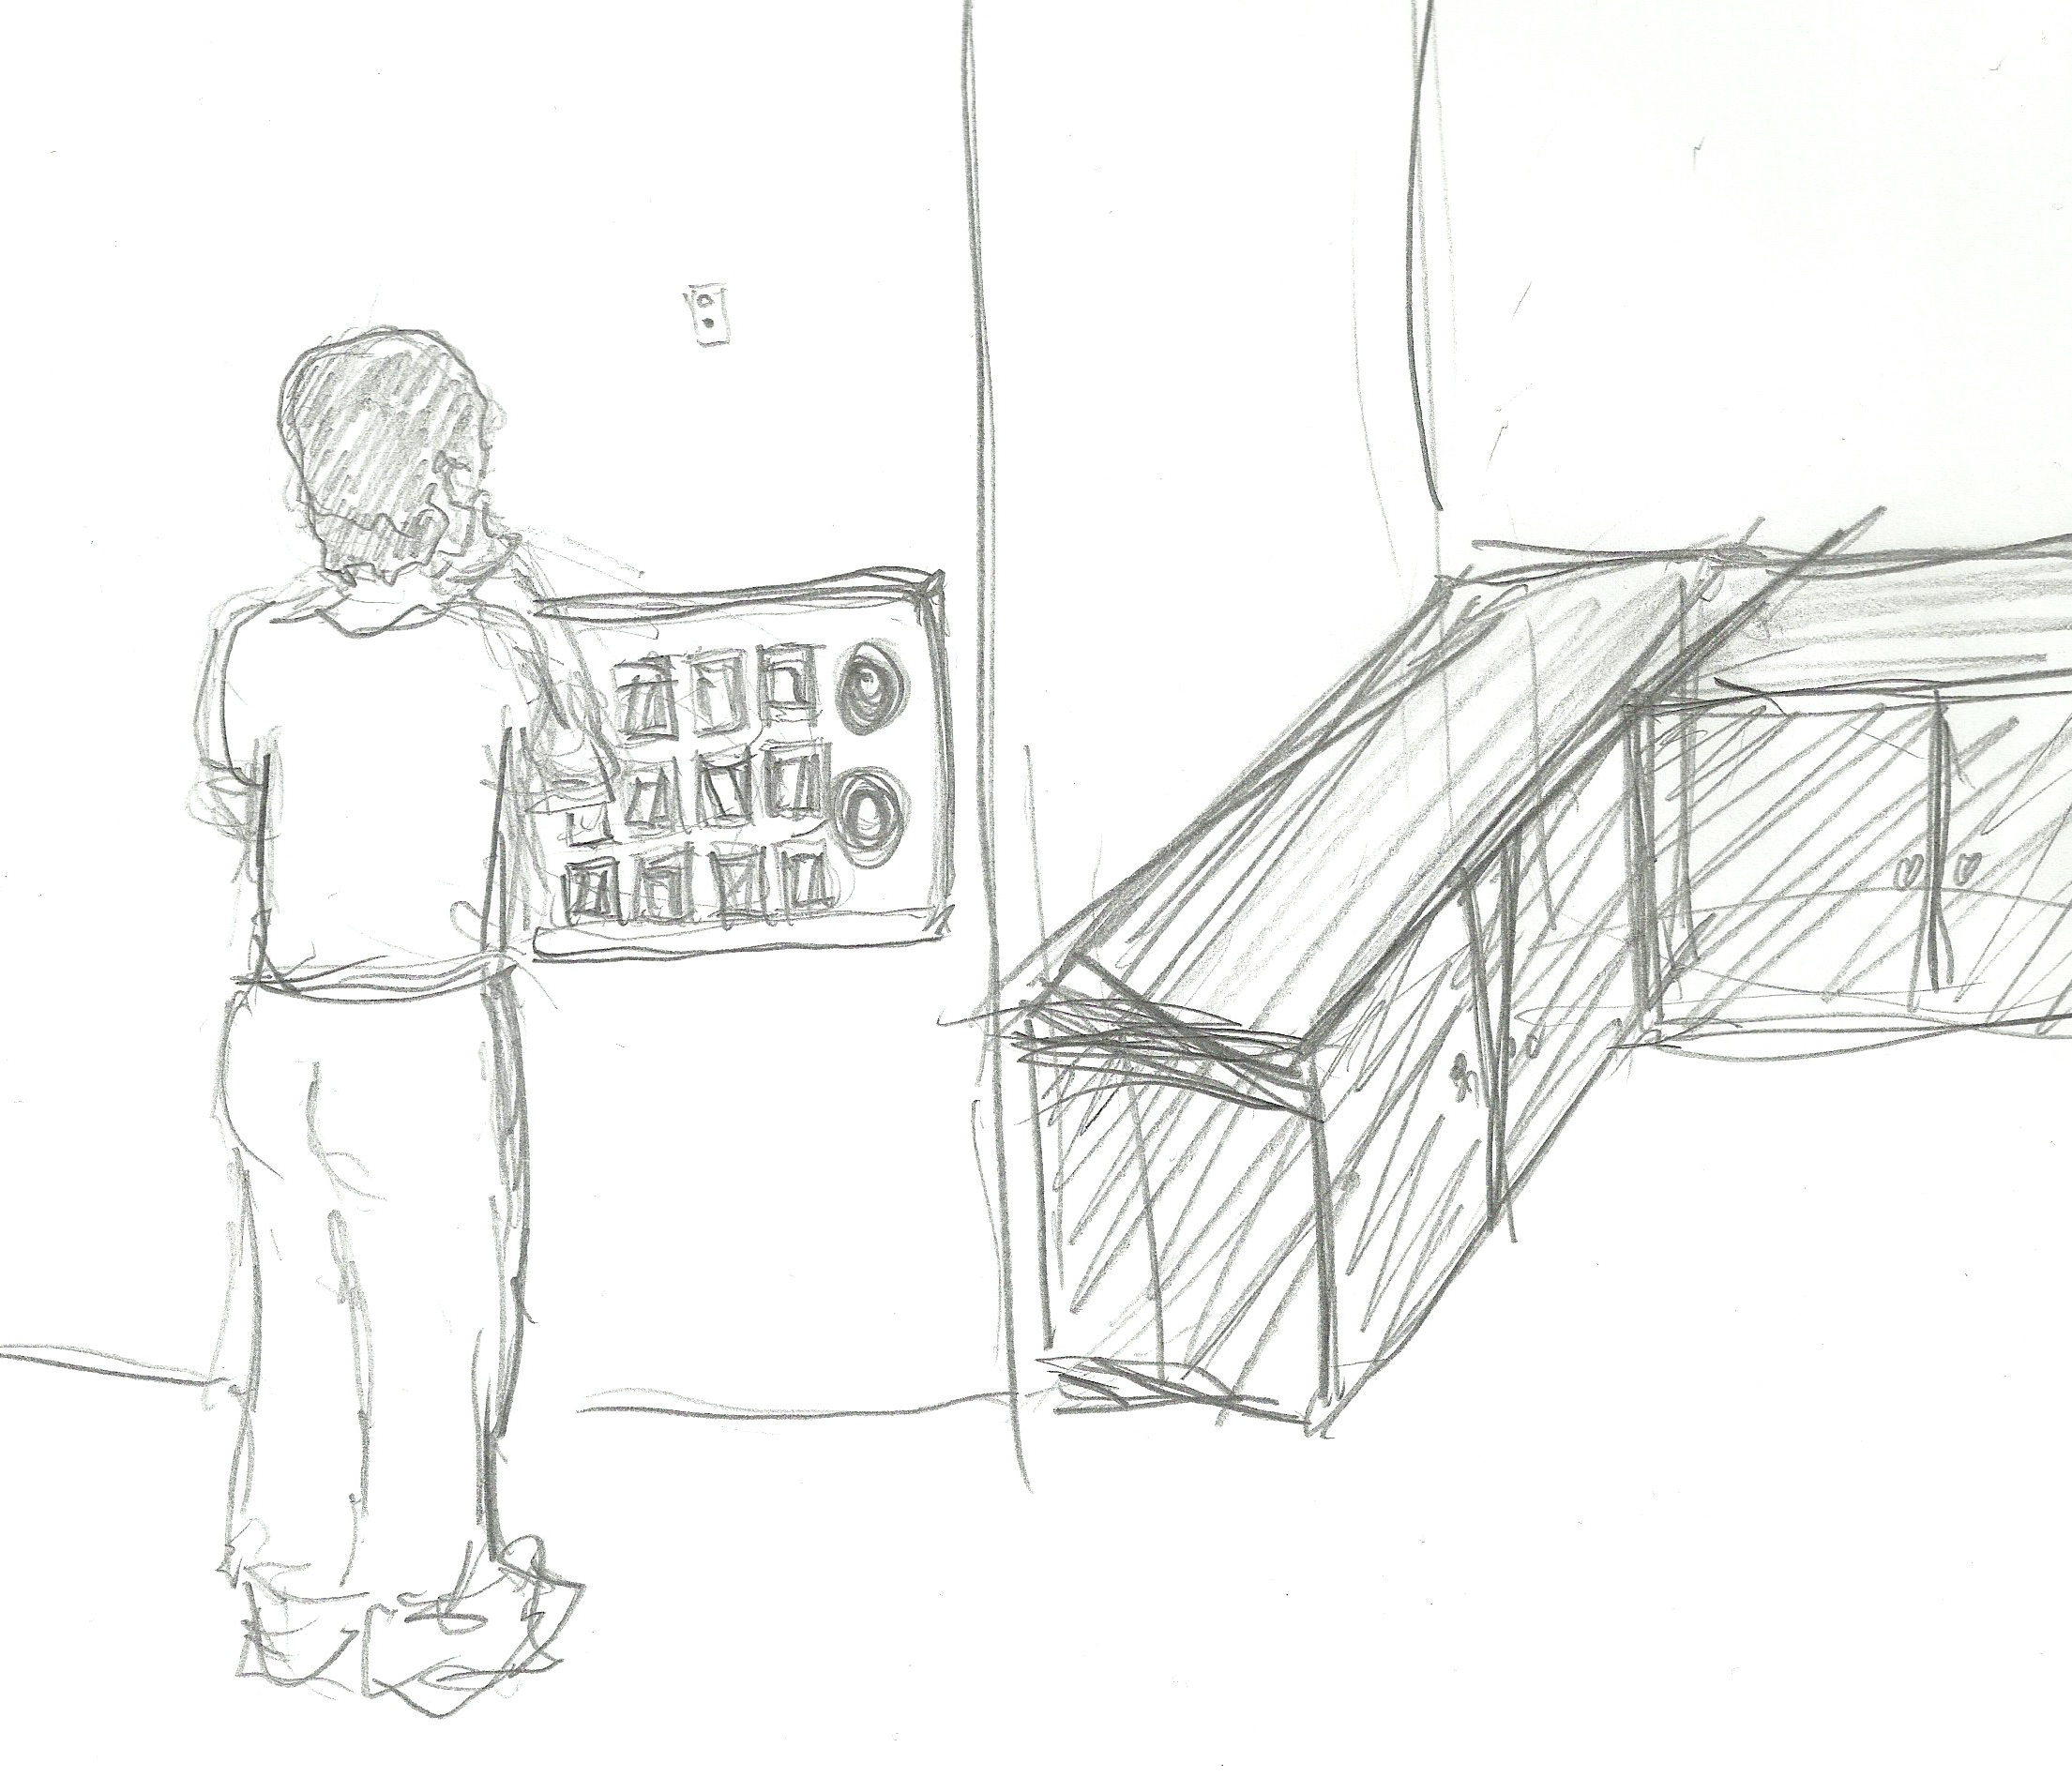
\includegraphics[scale=0.4]{fig/buttons}
\caption{Kommunikasjonssoner, gjenbrukt fra \citet{streitz05}. Displayet forandrer seg og tilbyr forskjellige interaksjonsmuligheter avhengig av hvilken sone brukeren befinner seg i.}
\label{commzones}
\end{figure}

Forskjellige interaksjonssoner beskrives av \citet{streitz05}. De omtaler interaksjonssonene omgivende, notifikasjon og interaksjon (figur \ref{commzones}). I den omgivende sonen kan brukeren oppfatte mønstere som vises på en vegg. Veggen sanser avstand til brukeren og viser mønstre ved å tenne et antall små, separate lyskilder. I notifikasjon vil personlige notifiseringsmønstre vises, og i interaksjon vil veggen vise spesielle mønstre og være interagerbar. Bruken av soner gir mulighet til å tilby forskjellige visninger og interaksjoner basert på avstand. Greenberg et al. omtaler fem målbare dimensjoner av \emph{proxemics}: \emph{Avstanden} mellom enheter og brukere virker naturlig, og passer godt inn med interaksjonssonene som er definert. \emph{Retning} gir et mål på vinkelen mellom enheter og brukere. Det finnes allerede enheter som gjør bruk av retning, for eksempel ved å skru seg av når folk ikke ser på dem. \emph{Bevegelse} omfatter forandring i distanse over tid. \emph{Identitet} beskriver en enhet i et gitt detaljnivå. \emph{Plassering} beskriver posisjonen til enheten, for eksempel i hvilket rom og hva konteksten rundt rommet er. \emph{Proxemics} kan i sin helhet være med på å tilby en mer naturlig interaksjon med enhetene våre og kan kanskje være det neste steget for utviklingen av interaksjonsapplikasjoner.

\subsubsection*{Gester}
En annen interaksjonsform det forskes på er gesturer. Dette er nok et forsøk på å tilby en mer naturlig interaksjon med datamaskinen. Kroppsspråket er tross alt en stor del av mellommenneskelig kommunikasjon, så hvorfor ikke forsøke å utvide det til kommunikasjon mellom menneske og maskin. \citet{homeos} omtaler en prosjektgruppe som utvidet HomeOS-systemet til å forstå gesturer, ved bruk av Kinect-kameraet. Det finnes mange prosjekter på nettet som har brukt Kinect til å skape systemer som forstår både gesturer og tale\footnote{Et godt dokumentert eksempelprosjekt som benytter Kinect's datasyn og talegjenkjenning: http://www.codeproject.com/Articles/715858/Home-Automation-with-Microsoft-Kinect-Point-Cloud, hentet des 2014.}. Ulempen med denne formen for gesturgjenkjenning er de samme som med sensorovervåking gjennom kameraer (kapittel 3.1): følelsen av overvåking og sikker håndtering av sensitive data. 

Det finnes andre, mindre påtrengende metoder for å detektere gesturer. Infrarøde gestur-sensorer kan tilby en kontaktløs interaksjon med det smarte hjemmet\footnote{SparkFun RGB and Gesture Sensor. Denne brikken kan måle lys, farge, avstand og gesturer: https://www.sparkfun.com/products/12787, hentet des 2014.}. Sensoren sender ut infrarøde signaler og mottar refleksjonen fra brukerens hånd. Mikrokontrolleren må så tolke disse verdiene til en gestur. Systemet kan dermed trenes med teknikker fra maskinlæring til å klassifisere og tolke forskjellige gesturer til å forskjellige kommandoer. Det infrarøde signalet reflekteres effektivt kun ut til en avstand på noen titalls centimeter. Dette blir dermed en mye mindre påtrengende metode enn bruk av video. Et bruksområde for gesturer kan være å be om det neste steget i en oppskrift, uten å måtte trykke på en touch-skjerm mens hendene er tilskitnet med mat. Det kan også være aktuelt å kombinere gesturer med en annen interaksjonsform, som tale. Et multimodalt brukergrensesnitt kan forbedre systemets nøyaktighet i tolkningen av kommandoene og avklare usikkerhet og misforståelser.

{\subsubsection{Hjemmet som en personlig assistent}
De fleste av oss har tilgang til en såkalt personlig assistent på smarttelefonen. På Android (og gjennom nettlesere) har man \emph{Google Now} og på iOS har man Apple's \emph{Siri}. Begge produktene er intelligente, personlige assistenter som tilbyr et brukergrensesnitt for naturlig språk hvor man kan få svar på spørsmål, anbefalinger og utførelser av handlinger gjennom web-tjenester. Begge tilpasser seg brukeren over tid og forsøker å levere individuelt tilpassede resultater.

I januar 2014 presenterte Intel et headset som i framtiden skal utfordre de personlige assistente fra Apple og Google, og de kaller det \emph{Jarvis}\footnote{http://www.theinquirer.net/inquirer/news/2325465/intels-jarvis-headset-will-take-on-apples-siri-and-google-glass-by-working-offline, hentet des 2014.}. Intel's fordel vil være at talegjenkjenningen utføres i headsettet, på den nye \emph{Edison-modulen}\footnote{http://www.intel.com/content/www/us/en/do-it-yourself/edison.html, hentet des 2014.}. Dermed fungerer den personlige assistenten selv når man ikke har kontakt med internettet. Når man kan unngå å sende forespørselen på en rundtur over nettet, for prosessering og analyse et annet sted, spares det mye tid og man unngår forsinkelsen som gjør dagens eksisterende systemer vanskelige å bruke. Science fiction inspirer ofte teknologisk utvikling og Intel's valg av navn er en klar referanse til datasystemet \emph{J.A.R.V.I.S.} fra \emph{Iron Man-filmene}\footnote{http://marvel-movies.wikia.com/wiki/J.A.R.V.I.S., hentet des 2014.}. Dette programmet styrer heltens smart hjem og kontrollerer alt der, som innemiljø og sikkerhet. Samtidig fungerer det som en personlig assistent og tilbyr hjelp med informasjonsgjenfinning og planlegging. Systemet interageres med gjennom touch-skjermer, talegjenkjenning, syntesert tale, holografi og robotikk. Så hvordan kan en slik personlig assistent som ikke bare tilbyr informasjon, men som selv utfører avanserte oppgaver, implementeres?

Mange webtjenester som folk flest bruker i dag, som kalendere, værkilder og trafikkdata, tilbyr også muligheten til å spørre kildene programmatisk gjennom API'er (\emph{application programming interfaces}. Dermed kan det smarte hjemmet kombinere sensordata fra huset med webtjenester. Basert på data fra kalendere, vær, trafikk og brukerens preferanser kan det smarte hjemmet for eksempel kalkulere at brukeren har tid til å gå til sitt første møte for dagen. Dersom brukeren svarer bekreftende på et slikt forslag kan systemet planlegge reiseruten til møtestedet og laste ned nødvendige kartdata til brukerens mobiltelefon. Dette er funksjonalitet som kan implementeres i dag. Et mer avansert scenario, der hjemmet gjør større, proaktive handlinger på brukerens vegne, og har muligheten for å hente informasjon fra informasjonskilder brukeren ikke kjenner til krever en annen teknologi. Dette er teknologi som eksisterer, men ennå ikke er utbredt. \citet{semantic01} legger grunnlaget for det neste steget i webbens evolusjon, en semantiske web. Dersom hjemmet for eksempel skal kunne kjøpe ønskede billetter på brukerens vegne trengs det en felles, vidspredt platform for kunnskapsrepresentasjon og en felles forståelse for beskrivelsen av og sammenhengene mellom informasjon. Først da kan systemer kommunisere seg i mellom uten menneskelig intervensjon på en trygg og sikker måte. En semantisk web foreslår \emph{Resource Description Framework (RDF)} for å representere kunnskap og avtalte ontologier for å beskrive informasjon og sammenhenger. At data er lagret i RDF gjør det enkelt å ta kontakt med mange forskjellige datakilder samtidig og lage kompliserte spørringer. Ontologiene gjør at det oppnås en felles forståelse for hvordan kunnskap henger sammen. Modellen som en helhet klargjør for å lage automatiserte agenter som kan kommunisere seg i mellom og utføre arbeid og transaksjoner som tidligere trengte sterk menneskelig innblanding, som å ta kontakt med en selgeragent hos en billettjeneste og bestille billetter på brukerens vegne.

\subsubsection*{Video -problemer med personvern}
Video gir potensialet for å realisere virkelig smarte systemer som kan motta kommandoer gjennom gesturer, forstå hjemmets tilstand, gjenkjenne beboerenes aktiviteter og kanskje til forstå kontekst. Video produserer store datamengder og dette gir en større teknisk utfordring med henhold til lagringsplass og datautvinning enn bruk av enklere sensorer. Heldigvis er det utviklet mange gode teknikker for å analysere bilder og desto mer tid som går desto større blir lagringskapasitetene våre.

Et eksempelprosjekt som blant annet gjør bruk av video er \emph{Placelab-prosjektet}, beskrevet av \citet{placelab05}. I sin studie gjorde de blant annet bruk av ni infrarøde kameraer, ni fargekameraer og atten mikrofoner spredd gjennom en leilighet. Ved bruk av bildebehandlingsalgortimer kunne de velge hvilke av datastrømmene som best fanget beboerens oppførsel til et gitt tidspunkt.

Baksiden av videomedaljen er beskyttelse av personvernet og brukerenes følelse av å opprettholde et privatliv i hjemmet. Intuitivt kan man forestille seg at de færreste brukere i utgangspunktet ønsker kameraer som filmer dem overalt i hjemmet. Selv dersom det kunne garanteres at informasjonen aldri forlot hjemmet, eller at den kun blir lagret i en kort tidsperiode, vil tilsynelatende konstant overvåking være noe mange vil sette et stort spørsmåltegn ved. I overvåkningssamfunnet i George Orwell's \emph{1984} har hver leilighet en skjerm med tilhørende kameraovervåking som kan se stort sett alt som foregår. I dette samfunnet har befolkningen over tid godtatt overvåkningen, i den tro at det er til deres eget beste. I vår verden ser ut til at folk flest godtar dagens nivå av overvåkning gjennom loggførte posisjonsdata fra smarttelefoner, søkeord og forflytninger med fly og bil. Men introduksjonen av videokameraer i stuene vil kanskje oppleves som for mye, selv hvis informasjonen kun holdes og brukes lokalt.

%%=========================================
\subsubsection*{Problemformulering}
asd

%%=========================================
\subsection{Mål}
Basert på dette arbeidet ønsker jeg å jobbe videre med en masteroppgave som omhandler brukergrensesnitt i forbindelse med smarte hjem. Spesielt vil det være spennende å utforske alternativer til touch-skjermer og laptoper for å kommunisere med hjemmet. Basert på resultatene fra brukerstudiene og Rogers argumenter presentert i kapittel seks er jeg overbevist om at vi ikke ønsker et proaktivt hjem hvor brukerene lener seg tilbake og lar omgivelsene ta seg av alt. Jeg tror vi ønsker å bli engasjert og at spennende og utfordrende brukergrensesnitt kan være med på å skape en ny renessanse for interaksjonen med datamaskinen.

Våren 2015 vil jeg jobbe med bruken av gesturer for å interagere med et smart hjem. Dette kan bli i en multimodal setting der man også gjør bruk av touch-skjermer og/eller tale. Oppgaven peker mot at mange mennesker ikke ønsker kameraer i hjemmene sine. Da passer i steden for de infrarøde gestur-sensorer presentert i kapittel seks godt. Arbeidet kan omhandle faktiske brukere og utforske om gesturer er en verdifull måte å interagere på. En annen tilnærming kan være å bruke maskinlæring for å få systemet til å lære å tolke ulike gesturer gjennom klassifisering. Et tredje alternativ er å kombinere gesturer med annen input og se om multimodal interaksjon kan forbedre systemets nøyaktighet og avklare misforståelser.
Hovedmålene for dette prosjektet er å
\begin{enumerate}
\item Utforske bruken av enkle gestesensorer kombinert med talegjenkjenning som en effektiv og naturlig interaksjon med hjemmet.
\item Utforske kontekstdrevne brukergrensesnitt.
\end{enumerate}

%%=========================================
\subsection{Begrensninger}
asd

%%=========================================
\subsection{Rapportens struktur}
Dette introduksjonskapitellet etterfølges av fire interaksjonsprosjekter, samt et avsluttende kapittel. 